\documentclass[12pt]{article}
\usepackage[T2A]{fontenc}
\usepackage[utf8]{inputenc}
\usepackage{multirow}
\usepackage{caption}
\usepackage{subcaption}
\usepackage{amsmath}
\usepackage{changepage}
\usepackage{graphicx}
\usepackage{float}
\usepackage[english,russian]{babel}
\usepackage{amsmath, amsfonts, amssymb, amsthm, mathtools}
\usepackage{xcolor}
\usepackage{array}
\usepackage{hyperref}
\usepackage[top = 1.5cm, left = 1.5 cm, right = 1.5 cm, bottom = 3 cm]{geometry}
\graphicspath{ {./images/} }
 
\title{Измерение интенсивности радиационного фона}
\author{Шахматов Андрей, Б02-304}
\date{\today}
  
\begin{document}
\begin{titlepage}
    \begin{center}
        {\large МОСКОВСКИЙ ФИЗИКО-ТЕХНИЧЕСКИЙ ИНСТИТУТ (НАЦИОНАЛЬНЫЙ ИССЛЕДОВАТЕЛЬСКИЙ УНИВЕРСИТЕТ)}
    \end{center}
    \begin{center}
        {\large Физтех-школа физики и исследований им. Ландау}
    \end{center}
    
    
    \vspace{3cm}
    {\huge
        \begin{center}
            \textbf{Измерение интенсивности радиационного фона}
        \end{center}
    }
    \vspace{2cm}
    \begin{flushright}
        {\LARGE Автор:\\ Шахматов Андрей Юрьевич \\
            \vspace{0.2cm}
            Б02-304}
    \end{flushright}
    \vspace{7 cm}
    \begin{center}
        Долгопрудный 2023
    \end{center}
\end{titlepage}

% \maketitle

\begin{abstract}
    Используя счётчик Гейгера-Мюллера, измерена интенсивность космического излучения с поверхности Земли на 
    географических координатах ($55^\circ$ с. ш. $37^\circ$ в. д). Показано, что среднеквадратичное отклонение, полученное экспериментально,
    соответствует среднеквадратичному отклонению, вычисленному теоретически. Установлено, что средние значения и дисперсии 
    пропорциональны длине интервала разбиения. Это может свидетельствовать о том, что распределение интенсивности частиц космического 
    излучения соответствует распределению Пуассона.
\end{abstract}

\tableofcontents

\section{Введение}

Измерение интенсивности космического излучения, попадающего на Землю, является важной задачей современной астрофизики. Считается, что
распределением, соответствующим дискретным значениям с фиксированным средним является распределение Пуассона $w_n(\overline{n}) = \frac{{\overline{n}}^{n}}{n!}e^{-\overline{n}}$, 
где $\overline{n}$ - среднее значение выборки. Однако неизвестно, подчиняются ли ему данные, характеризующие интенсивность космического излучения.
Цель настоящей работы заключалась в измерении интенсивности космического изучения на Земле в точке с координатами ($55^\circ$ с. ш. $37^\circ$ в. д)
и определении, соответствует ли оно распределению Пуассона.

\section{Методика}
\subsection{Методика проведения измерений}
Для измерения интенсивности космического излучения используется счётчик Гейгера-Мюллера (прибор СТС-6). Он представляет собой сосуд,
наполненный газом, с двумя электродами. При пролёте частицы излучения выбивают электроны из газа, которые из-за действия сильного электрического
поля, ускоряются и выбивают вторичные электроны, таким образом создаётся лавинный эффект. Контроллер счётчика способен уловить
изменение тока и зарегистрировать частицу излучения.
\subsection{Методика анализа полученных результатов}
Чтобы проверить, соответствует ли распределение интенсивности космического излучения распределению Пуассона, можно произвести разбиение 
данных на несколько интервалов. Из теоретических расчётов \cite{LabBook} следует, что среднеквадратичные отклонения отдельных измерений
$\sigma_i$ связаны со средним значением выборки $\overline{n}$ выражением 
\begin{equation}\label{eq:6}
    \sigma_i = \sqrt{n_i} = \sqrt{\overline{n}}.
\end{equation}
Отношения среднеквадратичных отклонений $\frac{\sigma_{N_1}}{\sigma_{N_2}}$ для различных интервалов разбиений с числом отсчётов 
$N_1, N_2$ связаны со средними значениями выборок $\overline{n_1}$ и $\overline{n_2}$ выражением
\begin{equation}\label{eq:7}
    \frac{\sigma_{N_1}}{\sigma_{N_2}} = \sqrt{\frac{\overline{n_1}}{\overline{n_2}}} = \sqrt{\frac{N_2}{N_1}}.
\end{equation}
Среднеквадратичное отклонение среднего значения $\sigma_{\overline{n}}$ выражается через число отсчётов $N$ и среднее значение 
$\overline{n}$:
\begin{equation}\label{eq:8}
    \sigma_{\overline{n}} = \frac{\sigma_i}{\sqrt{N}} = \sqrt{\frac{\overline{n}}{N}}.
\end{equation}
Относительная ошибка среднего значения $\epsilon_{\overline{n}}$ выражается через число отсчётов $N$ и среднее значение 
$\overline{n}$:
\begin{equation}\label{eq:9}
    \epsilon_{\overline{n}} = \frac{\sigma_{\overline{n}}}{\overline{n}} = \frac{1}{\sqrt{\overline{n}N}}.
\end{equation}
Из формулы~\ref{eq:9} следует, что относительная ошибка среднего не зависит от числа разбиений и уменьшается только при увеличении
общего числа измерений.
Соответствие результатов эксперимента значениям, полученным из формул \ref{eq:6}, \ref{eq:7}, \ref{eq:8}, \ref{eq:9},
может свидетельствовать о соответствии экспериментально полученного распределения распределению по Пуассону. 

\section{Результаты и их анализ}
В эксперименте время накопления счётчиком Гейгера-Мюллера количества зарегистрированных частиц составляло 1 с. За время проведения эксперимента
было накоплено 4000 точек, каждая длительностью 1 с.
Вычислено среднее значение ${\overline{n}}_1 = 1.2515$ и среднеквадратичное отклонение ${\sigma}_1 = 1.1367$ полученного распределения.
А также рассчитано среднеквадратичное отклонение ${\sigma_{poisson}}_1 = 1.1187$, вычисленное из предположения, что распределение является 
распределением Пуассона (Формула \ref{eq:6}). Соответствие значения ${\overline{n}}_1$ значению ${\sigma_{poisson}}_1$ может 
свидетельствовать о соответствии полученного распределения распределению Пуассона.

Из графика распределения (график \ref{fig:1}) установлено, что распределение визуально соответствует Пуассоновскому.
\begin{figure}[H]
    \begin{center}
        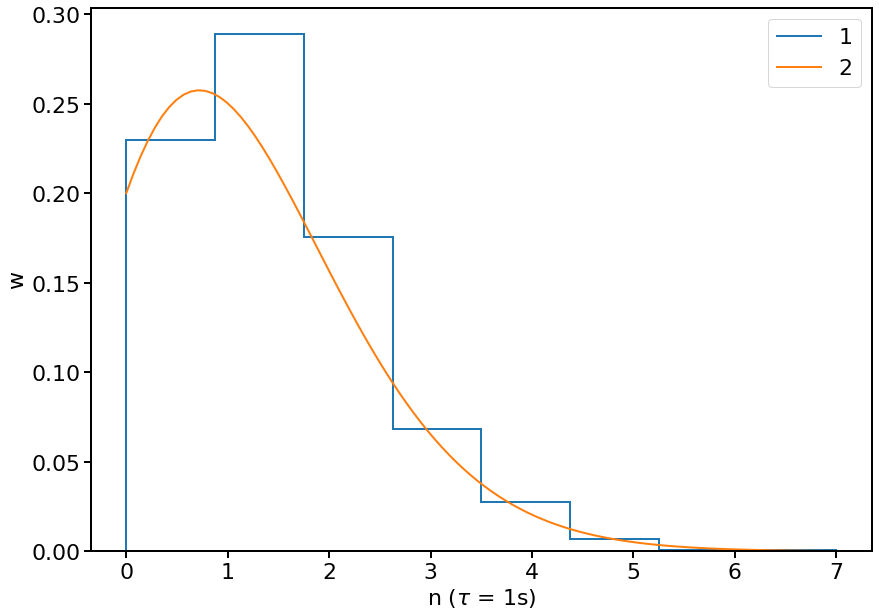
\includegraphics[width=0.7\textwidth]{gr1}
    \end{center}
    \caption{Распределение количества частиц, зарегистрированных счётчиком Гейгера-Мюллера СТС-6, с усреднением по интервалу разбиения
        равным $1$с. По оси $w$ отложена доля количества частиц, зарегистрированных за интервал разбиения. По оси $n$ отложены
        количества частиц, зарегистрированных за интервал разбиения. 1 - экспериментальное распределение, 2 - аппроксимирующее распределение Пуассона.}
    \label{fig:1}
\end{figure}
Для дальнейшего анализа распределения было произведено разбиение данных по интервалам 10, 20, 40 секунд (Таблицы \ref{tab:1}, \ref{tab:2}, \ref{tab:3})
Гистограммы для для соответствующих разбиений представлены на рисунке \ref{fig:2}.
\begin{figure}[H]
    \begin{center}
        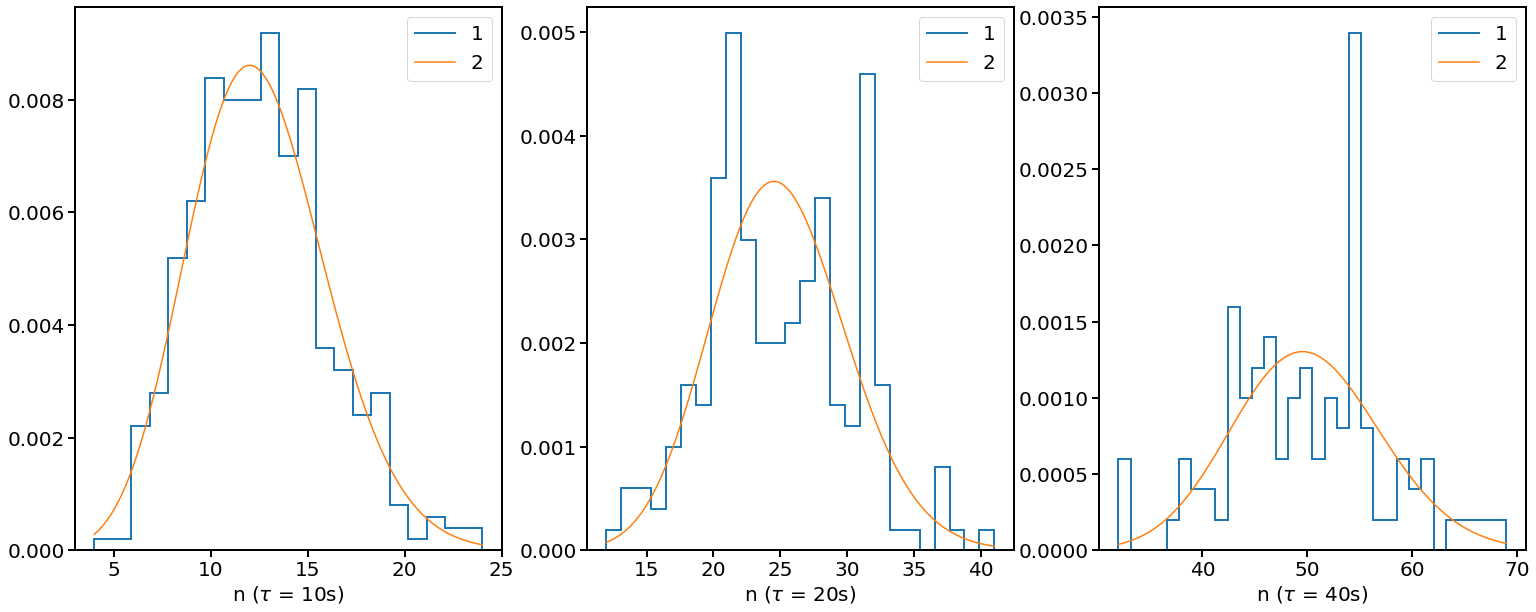
\includegraphics[width=\textwidth]{gr2}
    \end{center}
    \caption{Распределения количества частиц, зарегистрированных счётчиком Гейгера-Мюллера СТС-6, с усреднением по интервалам разбиения
        $10c, 20c$ и $40$с. По оси $w$ отложена доля количества частиц, зарегистрированных за интервал разбиения. 
        По оси $n$ отложены количества частиц, зарегистрированных за интервал разбиения. 1 - экспериментальное распределение, 
        2 - аппроксимирующее распределение Пуассона.}
    \label{fig:2}
\end{figure}
Из графика \ref{fig:2} можно сделать вывод, что распределение продолжает визуально соответствовать Пуассоновскому 
независимо от интервала измерения.

Для проведения сравнительного анализа распределений для двух интервалов разбиений построена совмещённая гистограмма для разбиений с 
числом разбиений $10$с и $40$с.

\begin{figure}[H]
    \begin{center}
        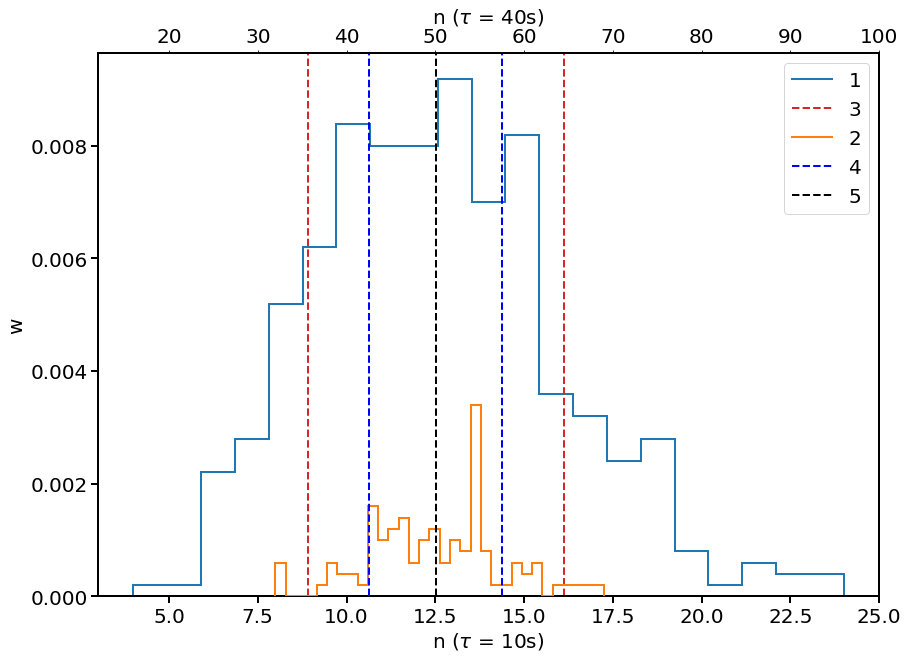
\includegraphics[width=0.7\textwidth]{gr3}
    \end{center}
    \caption{Распределения количества частиц, зарегистрированных счётчиком Гейгера-Мюллера СТС-6, с усреднением по интервалам разбиения
        $10$с и $40$с. По оси $w$ отложена доля количества частиц, зарегистрированных за интервал разбиения. 
        По оси $n$ отложены количества частиц, зарегистрированных за интервал разбиения. Разбиения построены на шкалах таким образом, 
        чтобы среднее значения обоих распределений совпадало. 1 - распределение с интервалом разбиения $10$с, 
        2 - распределение с интервалом разбиения $40$с, 3 - среднеквадратичное отклонение распределения с интервалом разбиения $10$с, 
        4 - среднеквадратичное отклонение распределения с интервалом разбиения $40$с, 5 - среднее обоих распределений}
    \label{fig:3}
\end{figure}
Графически установлено, что стандартное отклонение для $\tau = 40$с ($\sigma_{40} = 7.5$) примерно равно удвоенному значению
стандартного отклонения для $\tau = 10$с ($\sigma_{10} = 3.6$), что соответствует теории (Формула \ref{eq:6}).

Для того чтобы проверить соответствие экспериментальных распределений на различных интервалах разбиений Пуассоновскому распределению 
рассчитано количество частиц попадающих в интервал $\sigma$ и $2\sigma$, полученные значения сравнены с рассчитанными теоретически\cite{LabBook}
(Таблица \ref{tab:4}).
\begin{table}[H]
    \begin{tabular}{|c|c|c|c|}
        \hline
        Интервал разбиений            & Стандартное отклонение      & Доля случаев, \% & Теоретическая оценка, \% \\
        \hline
        \multirow{2}{*}{$\tau$ = 1с}  & ${\pm}{\sigma} = \pm1.14$   & 58               & 68                       \\ 
                                      & ${\pm}{2\sigma} = \pm2.27$  & 95               & 95                       \\
        \hline
        \multirow{2}{*}{$\tau$ = 10с} & ${\pm}{\sigma} = \pm3.60$   & 73               & 68                       \\ 
                                      & ${\pm}{2\sigma} = \pm7.20$  & 97               & 95                       \\
        \hline
        \multirow{2}{*}{$\tau$ = 20с} & ${\pm}{\sigma} = \pm5.45$   & 63               & 68                       \\ 
                                      & ${\pm}{2\sigma} = \pm10.89$ & 96               & 95                       \\
        \hline
        \multirow{2}{*}{$\tau$ = 40с} & ${\pm}{\sigma} = \pm7.50$   & 61               & 68                       \\ 
                                      & ${\pm}{2\sigma} = \pm15.00$ & 93               & 95                       \\
        \hline
        
    \end{tabular}
    \caption{Доли попадания количества частиц, зарегистрированных за интервал разбиения $\tau$ в окрестности ${\pm}{\sigma}$ и ${\pm}{2\sigma}$
        от среднего значения соответствующего распределения.}
    \label{tab:4}
\end{table}
Из таблицы \ref{tab:4} следует, что независимо от интервала разбиения доля случаев, полученная экспериментально, 
совпадает с теоретической оценкой.

Расчитаны стандартная ошибка (Формула \ref{eq:8}) и относительная ошибка (Формула \ref{eq:9}).
Значения стандартной и относительной ошибок для различных интервалов разбиений и количеством отсчётов $N$ представлены в таблице \ref{tab:5}.
\begin{table}[H]
    \begin{center}
        \begin{tabular}{|c|c|c|c|}
            \hline
            $N$  & Среднее значение $\overline{n}$ & Стандартная ошибка $\sigma_{\overline{n}_N}$ & Относительная ошибка $\epsilon_{\overline{n}_N}$ \\
            \hline
            4000 & 1.25                             & 0.02                                          & 0.014                                             \\
            400  & 12.5                             & 0.2                                           & 0.014                                             \\
            200  & 25.0                             & 0.4                                           & 0.015                                             \\
            100  & 50.1                             & 0.8                                           & 0.015                                             \\
            \hline
        \end{tabular}
    \end{center}
    \caption{Значения среднего, стандартной ошибки и относительной ошибки распределения количества частиц для различных интервалов разбиений}
    \label{tab:5}
\end{table}
Теоретически предсказанная относительная ошибка составила $\sigma_{\overline{n}} = \frac{1}{\sqrt{4000\cdot1.25}} = 0.014$.
Из полученных данных следует, что относительная ошибка не зависит от интервала разбиения данных, а также соответствует теоретической оценке.

\section{Выводы}
Cреднее значение интенсивности космического излучения оказалось равно $(1.25 \pm 0.02)\frac{\textrm{частиц}}{\textrm{с}}$.
При этом отношение средних значений интенсивности и их дисперсий для различных интервалов разбиения оказалось равно отношению длительностей 
соответствующих интервалов разбиения, что является характерным признаком распределения Пуассона.
Отсюда следует, что распределение интенсивности космического излучения может подчиняться распределению Пуассона.

\section{Использованная литература}
\begin{thebibliography}{9}
    \bibitem{LabBook}
    Лабораторный практикум по общей физике, Том 1, под редакцией А. Д. Гладуна
\end{thebibliography}

\section{Приложения}
\subsection{Измерения количества частиц за определённые интервалы времени} \label{sec:app_1}
\begin{table}[H]
    \begin{center}
        \begin{tabular}{|l|r|r|r|r|r|r|r|r|r|r|r|r|r|r|r|r|r|r|r|r|}
            \hline
               & 0  & 1  & 2  & 3  & 4  & 5  & 6  & 7  & 8  & 9  & 10 & 11 & 12 & 13 & 14 & 15 & 16 & 17 & 18 & 19 \\
            \hline
            0  & 15 & 14 & 18 & 15 & 14 & 19 & 9  & 13 & 14 & 9  & 6  & 16 & 11 & 4  & 14 & 15 & 10 & 15 & 18 & 16 \\
            1  & 12 & 15 & 13 & 9  & 19 & 13 & 7  & 14 & 13 & 14 & 16 & 14 & 12 & 19 & 11 & 13 & 18 & 13 & 23 & 15 \\
            2  & 14 & 12 & 9  & 8  & 11 & 11 & 15 & 17 & 10 & 12 & 9  & 9  & 14 & 15 & 17 & 16 & 14 & 9  & 12 & 19 \\
            3  & 9  & 13 & 15 & 22 & 13 & 11 & 12 & 20 & 15 & 13 & 15 & 9  & 16 & 10 & 14 & 12 & 12 & 16 & 10 & 18 \\
            4  & 14 & 13 & 12 & 7  & 13 & 18 & 11 & 11 & 17 & 11 & 20 & 11 & 13 & 9  & 17 & 15 & 10 & 17 & 13 & 15 \\
            5  & 13 & 15 & 10 & 11 & 7  & 13 & 9  & 12 & 8  & 10 & 18 & 15 & 16 & 9  & 11 & 15 & 14 & 14 & 16 & 12 \\
            6  & 12 & 16 & 13 & 8  & 8  & 24 & 11 & 12 & 9  & 11 & 15 & 15 & 14 & 12 & 15 & 13 & 11 & 8  & 10 & 9  \\
            7  & 13 & 12 & 12 & 15 & 11 & 16 & 10 & 10 & 16 & 13 & 20 & 17 & 16 & 16 & 17 & 11 & 23 & 10 & 9  & 11 \\
            8  & 8  & 12 & 7  & 18 & 17 & 11 & 6  & 9  & 11 & 19 & 14 & 10 & 8  & 9  & 7  & 13 & 13 & 9  & 8  & 8  \\
            9  & 15 & 16 & 10 & 10 & 9  & 15 & 8  & 15 & 10 & 14 & 19 & 13 & 12 & 14 & 11 & 8  & 9  & 10 & 10 & 10 \\
            10 & 22 & 10 & 10 & 10 & 7  & 10 & 15 & 22 & 20 & 9  & 7  & 13 & 9  & 11 & 13 & 11 & 18 & 12 & 7  & 13 \\
            11 & 11 & 7  & 12 & 15 & 12 & 15 & 12 & 11 & 14 & 6  & 8  & 15 & 15 & 13 & 12 & 13 & 13 & 7  & 14 & 16 \\
            12 & 15 & 18 & 12 & 13 & 11 & 10 & 19 & 14 & 15 & 12 & 12 & 8  & 15 & 8  & 13 & 8  & 10 & 11 & 17 & 5  \\
            13 & 11 & 12 & 6  & 12 & 9  & 8  & 17 & 9  & 6  & 8  & 10 & 8  & 17 & 10 & 12 & 9  & 12 & 11 & 9  & 17 \\
            14 & 10 & 12 & 12 & 8  & 10 & 10 & 10 & 13 & 14 & 17 & 14 & 7  & 10 & 15 & 11 & 19 & 15 & 10 & 13 & 10 \\
            15 & 10 & 16 & 14 & 15 & 19 & 18 & 13 & 15 & 9  & 12 & 12 & 11 & 10 & 6  & 14 & 17 & 10 & 8  & 14 & 13 \\
            16 & 11 & 12 & 16 & 15 & 6  & 12 & 15 & 10 & 11 & 18 & 13 & 12 & 13 & 18 & 17 & 14 & 11 & 11 & 13 & 13 \\
            17 & 6  & 8  & 9  & 10 & 15 & 11 & 10 & 14 & 11 & 6  & 10 & 11 & 19 & 12 & 7  & 7  & 19 & 16 & 19 & 13 \\
            18 & 14 & 13 & 19 & 14 & 19 & 13 & 15 & 8  & 9  & 14 & 24 & 17 & 15 & 12 & 14 & 14 & 11 & 21 & 8  & 10 \\
            19 & 14 & 14 & 8  & 7  & 13 & 11 & 12 & 8  & 9  & 10 & 15 & 13 & 13 & 9  & 11 & 13 & 6  & 6  & 13 & 8  \\
            \hline
        \end{tabular}
    \end{center}
    \caption{Количества частиц, зарегистрированных счётчиком Гейгера-Мюллера, с усреднением по интервалу 10 с}
    \label{tab:1}
\end{table}
\begin{table}[H]
    \begin{center}
        \begin{tabular}{|l|r|r|r|r|r|r|r|r|r|r|}
            \hline
               & 0  & 1  & 2  & 3  & 4  & 5  & 6  & 7  & 8  & 9  \\
            \hline
            0  & 29 & 33 & 33 & 22 & 23 & 22 & 15 & 29 & 25 & 34 \\
            1  & 27 & 22 & 32 & 21 & 27 & 30 & 31 & 24 & 31 & 38 \\
            2  & 26 & 17 & 22 & 32 & 22 & 18 & 29 & 33 & 23 & 31 \\
            3  & 22 & 37 & 24 & 32 & 28 & 24 & 26 & 26 & 28 & 28 \\
            4  & 27 & 19 & 31 & 22 & 28 & 31 & 22 & 32 & 27 & 28 \\
            5  & 28 & 21 & 20 & 21 & 18 & 33 & 25 & 26 & 28 & 28 \\
            6  & 28 & 21 & 32 & 23 & 20 & 30 & 26 & 28 & 19 & 19 \\
            7  & 25 & 27 & 27 & 20 & 29 & 37 & 32 & 28 & 33 & 20 \\
            8  & 20 & 25 & 28 & 15 & 30 & 24 & 17 & 20 & 22 & 16 \\
            9  & 31 & 20 & 24 & 23 & 24 & 32 & 26 & 19 & 19 & 20 \\
            10 & 32 & 20 & 17 & 37 & 29 & 20 & 20 & 24 & 30 & 20 \\
            11 & 18 & 27 & 27 & 23 & 20 & 23 & 28 & 25 & 20 & 30 \\
            12 & 33 & 25 & 21 & 33 & 27 & 20 & 23 & 21 & 21 & 22 \\
            13 & 23 & 18 & 17 & 26 & 14 & 18 & 27 & 21 & 23 & 26 \\
            14 & 22 & 20 & 20 & 23 & 31 & 21 & 25 & 30 & 25 & 23 \\
            15 & 26 & 29 & 37 & 28 & 21 & 23 & 16 & 31 & 18 & 27 \\
            16 & 23 & 31 & 18 & 25 & 29 & 25 & 31 & 31 & 22 & 26 \\
            17 & 14 & 19 & 26 & 24 & 17 & 21 & 31 & 14 & 35 & 32 \\
            18 & 27 & 33 & 32 & 23 & 23 & 41 & 27 & 28 & 32 & 18 \\
            19 & 28 & 15 & 24 & 20 & 19 & 28 & 22 & 24 & 12 & 21 \\
            \hline
        \end{tabular}
    \end{center}
    \caption{Количества частиц, зарегистрированных счётчиком Гейгера-Мюллера, с усреднением по интервалу 20 с}
    \label{tab:2}
\end{table}
\begin{table}[H]
    \begin{center}
        \begin{tabular}{|l|r|r|r|r|r|r|r|r|r|r|}
            \hline
              & 0  & 1  & 2  & 3  & 4  & 5  & 6  & 7  & 8  & 9  \\
            \hline
            0 & 62 & 55 & 45 & 44 & 59 & 49 & 53 & 57 & 55 & 69 \\
            1 & 43 & 54 & 40 & 62 & 54 & 59 & 56 & 52 & 52 & 56 \\
            2 & 46 & 53 & 59 & 54 & 55 & 49 & 41 & 51 & 51 & 56 \\
            3 & 49 & 55 & 50 & 54 & 38 & 52 & 47 & 66 & 60 & 53 \\
            4 & 45 & 43 & 54 & 37 & 38 & 51 & 47 & 56 & 45 & 39 \\
            5 & 52 & 54 & 49 & 44 & 50 & 45 & 50 & 43 & 53 & 50 \\
            6 & 58 & 54 & 47 & 44 & 43 & 41 & 43 & 32 & 48 & 49 \\
            7 & 42 & 43 & 52 & 55 & 48 & 55 & 65 & 44 & 47 & 45 \\
            8 & 54 & 43 & 54 & 62 & 48 & 33 & 50 & 38 & 45 & 67 \\
            9 & 60 & 55 & 64 & 55 & 50 & 43 & 44 & 47 & 46 & 33 \\
            \hline
        \end{tabular}
    \end{center}
    \caption{Количества частиц, зарегистрированных счётчиком Гейгера-Мюллера, с усреднением по интервалу 40 с}
    \label{tab:3}
\end{table}
\subsection{Таблицы для построения гистограмм}\label{sec:app_2}
\begin{table}[H]
    \begin{center}
        \begin{tabular}{|r|r|l|}
            \hline
            Число импульсов, n & Число случаев & Доля случаев, w \\
            \hline
            0                  & 1151          & 0.28775         \\
            1                  & 1448          & 0.362           \\
            2                  & 879           & 0.21975         \\
            3                  & 341           & 0.08525         \\
            4                  & 139           & 0.03475         \\
            5                  & 34            & 0.0085          \\
            6                  & 5             & 0.00125         \\
            7                  & 3             & 0.00075         \\
            \hline
        \end{tabular}
    \end{center}
    \caption{Данные для построения гистограммы \ref{fig:1}. Интервал разбиения равен 1с}
    \label{tab:6}
\end{table}
\begin{table}[H]
    \begin{center}
        \begin{tabular}{|r|r|l|}
            \hline
            Число импульсов, n & Число случаев & Доля случаев, w \\
            \hline
            4                  & 1             & 0.0025          \\
            5                  & 1             & 0.0025          \\
            6                  & 11            & 0.0275          \\
            7                  & 14            & 0.035           \\
            8                  & 26            & 0.065           \\
            9                  & 31            & 0.0775          \\
            10                 & 42            & 0.105           \\
            11                 & 40            & 0.1             \\
            12                 & 40            & 0.1             \\
            13                 & 46            & 0.115           \\
            14                 & 35            & 0.0875          \\
            15                 & 41            & 0.1025          \\
            16                 & 18            & 0.045           \\
            17                 & 16            & 0.04            \\
            18                 & 12            & 0.03            \\
            19                 & 14            & 0.035           \\
            20                 & 4             & 0.01            \\
            21                 & 1             & 0.0025          \\
            22                 & 3             & 0.0075          \\
            23                 & 2             & 0.005           \\
            24                 & 2             & 0.005           \\
            \hline
        \end{tabular}
    \end{center}
    \caption{Данные для построения гистограммы \ref{fig:2}. Интервал разбиения равен 10с}
    \label{tab:7}
\end{table}
\begin{table}[H]
    \begin{center}
        \begin{tabular}{|r|r|l|}
            \hline
            Число импульсов, n & Число случаев & Доля случаев, w \\
            \hline
            12                 & 1             & 0.005           \\
            14                 & 3             & 0.015           \\
            15                 & 3             & 0.015           \\
            16                 & 2             & 0.01            \\
            17                 & 5             & 0.025           \\
            18                 & 8             & 0.04            \\
            19                 & 7             & 0.035           \\
            20                 & 18            & 0.09            \\
            21                 & 12            & 0.06            \\
            22                 & 13            & 0.065           \\
            23                 & 15            & 0.075           \\
            24                 & 10            & 0.05            \\
            25                 & 10            & 0.05            \\
            26                 & 11            & 0.055           \\
            27                 & 13            & 0.065           \\
            28                 & 17            & 0.085           \\
            29                 & 7             & 0.035           \\
            30                 & 6             & 0.03            \\
            31                 & 12            & 0.06            \\
            32                 & 11            & 0.055           \\
            33                 & 8             & 0.04            \\
            34                 & 1             & 0.005           \\
            35                 & 1             & 0.005           \\
            37                 & 4             & 0.02            \\
            38                 & 1             & 0.005           \\
            41                 & 1             & 0.005           \\
            \hline
        \end{tabular}
    \end{center}
    \caption{Данные для построения гистограммы \ref{fig:2}. Интервал разбиения равен 20с}
    \label{tab:8}
\end{table}
\begin{table}[H]
    \begin{center}
        \begin{tabular}{|r|r|l|}
            \hline
            Число импульсов, n & Число случаев & Доля случаев, w \\
            \hline
            32                 & 1             & 0.01            \\
            33                 & 2             & 0.02            \\
            37                 & 1             & 0.01            \\
            38                 & 3             & 0.03            \\
            39                 & 1             & 0.01            \\
            40                 & 1             & 0.01            \\
            41                 & 2             & 0.02            \\
            42                 & 1             & 0.01            \\
            43                 & 8             & 0.08            \\
            44                 & 5             & 0.05            \\
            45                 & 6             & 0.06            \\
            46                 & 2             & 0.02            \\
            47                 & 5             & 0.05            \\
            48                 & 3             & 0.03            \\
            49                 & 5             & 0.05            \\
            50                 & 6             & 0.06            \\
            51                 & 3             & 0.03            \\
            52                 & 5             & 0.05            \\
            53                 & 4             & 0.04            \\
            54                 & 9             & 0.09            \\
            55                 & 8             & 0.08            \\
            56                 & 4             & 0.04            \\
            57                 & 1             & 0.01            \\
            58                 & 1             & 0.01            \\
            59                 & 3             & 0.03            \\
            60                 & 2             & 0.02            \\
            62                 & 3             & 0.03            \\
            64                 & 1             & 0.01            \\
            65                 & 1             & 0.01            \\
            66                 & 1             & 0.01            \\
            67                 & 1             & 0.01            \\
            69                 & 1             & 0.01            \\
            \hline
        \end{tabular}
    \end{center}
    \caption{Данные для построения гистограммы \ref{fig:2}. Интервал разбиения равен 40с}
    \label{tab:9}
\end{table}
\end{document}